\documentclass[UTF8]{ctexart}
\usepackage{amsmath}
\usepackage{graphicx}
\usepackage{float}
\usepackage{subfigure}
\usepackage{xeCJK}
\usepackage{hyperref}
\usepackage{algorithm2e}
\usepackage{amsfonts}
\usepackage{epsfig}
\usepackage{listings}
\usepackage{xcolor}
% 定义可能使用到的颜色

\definecolor{CPPLight}  {HTML} {686868}
\definecolor{CPPSteel}  {HTML} {888888}
\definecolor{CPPDark}   {HTML} {262626}
\definecolor{CPPBlue}   {HTML} {4172A3}
\definecolor{CPPGreen}  {HTML} {487818}
\definecolor{CPPBrown}  {HTML} {A07040}
\definecolor{CPPRed}    {HTML} {AD4D3A}
\definecolor{CPPViolet} {HTML} {7040A0}
\definecolor{CPPGray}  {HTML} {B8B8B8}
\lstset{
    columns=fixed,
    numbers=left,                                        % 在左侧显示行号
    frame=none,                                          % 不显示背景边框
    backgroundcolor=\color[RGB]{245,245,244},            % 设定背景颜色
    keywordstyle=\color[RGB]{40,40,255},                 % 设定关键字颜色
    numberstyle=\footnotesize\color{darkgray},           % 设定行号格式
    commentstyle=\it\color[RGB]{0,96,96},                % 设置代码注释的格式
    stringstyle=\rmfamily\slshape\color[RGB]{128,0,0},   % 设置字符串格式
    showstringspaces=false,                              % 不显示字符串中的空格
    language=c++,                                        % 设置语言
    morekeywords={alignas,continute,friend,register,true,alignof,decltype,goto,
    reinterpret_cast,try,asm,defult,if,return,typedef,auto,delete,inline,short,
    typeid,bool,do,int,signed,typename,break,double,long,sizeof,union,case,
    dynamic_cast,mutable,static,unsigned,catch,else,namespace,static_assert,using,
    char,enum,new,static_cast,virtual,char16_t,char32_t,explict,noexcept,struct,
    void,export,nullptr,switch,volatile,class,extern,operator,template,wchar_t,
    const,false,private,this,while,constexpr,float,protected,thread_local,
    const_cast,for,public,throw,std},
}

\graphicspath{{images/}}
\setCJKmonofont{Microsoft YaHei}

\title{\Huge{简易计算机的设计与实现}\\ \huge{西安交通大学\\软件学院\\数字逻辑综合实验}}
\author{\huge{}}
\date{\Huge{\today}}

\begin{document}
  \maketitle
  \vspace{12mm}
  \begin{flushright}
  \Large{
    \textbf{组\ \ \ \ \ 长} \makebox[6em][l]{\ 易\ \ \ 凯  2151601053}

    \textbf{成\ \ \ \ \ 员} \makebox[6em][l]{\ 庞建业  2151601012}

                        %\makebox[5em][l]{\ 朱禹宏  2151601019}

                        \makebox[6em][l]{\ 屈\ \ \ 松  2151601067}

                        \makebox[6em][l]{\ 邢贺宇  2151601070}

                        \makebox[6em][l]{\ 肖\ \ \ 飞  2150900084}

    \textbf{联系邮箱} \makebox[6em][l]{\ williamyi96@gmail.com}

    \textbf{联系电话} \makebox[6em][l]{\ 13772103675}

    \textbf{项目网站} \makebox[6em][l]{\ \small{https://github.com/WilliamYi96/SimpleComputer}}

    \textbf{提交日期} \makebox[6em][l]{\ \today}
    }
    \end{flushright}
    \newpage
    \tableofcontents
    \newpage

    \section{致谢}
    Give my sincere thanks to Teacher Zhang for his excellent teaching skills and serious altitude for our homework. Give my sincere thanks to some students who have helped us and who have inspired us when discussing with them. Give my sincere thanks to ourselves because we have overcome all difficulties and have successfully finished our digital logic assignments -- simple computer. Give my sincere thanks to those pioneers who have devoted themselves to writing immortal books. Give my sincere thanks to all the people sharing their ideas and harvests without pay in QA communities.

    衷心感谢张琴老师出色的教学风范以及严谨的治学态度,衷心感谢那些在讨论中帮助和启发我们的同学们,衷心感谢克服了种种困难最终完成了数字逻辑综合实验的我们,衷心感谢那些写了不朽著作为后人指明道路的先驱们,衷心感谢那些在问答社区无私奉献自己智慧成果的所有同仁!
    \newpage

    \section{关于本报告的说明}
    本实验报告是西安交通大学2015级软件工程系本科生以《数字逻辑专题实验》设计为契机进行的《简易计算机的设计与实现》。小组共有5人,分别为软件51班庞建业,软件53班易凯,软件54班屈松、邢贺宇和肖飞。小组成员之间分工明确,严格采取工程模块化的设计思想,务必追求严禁,考虑周全。经过接近两个月的设计与实现,最终于2017年6月末完成整体设计,并通过Quartus仿真以及验收。

    组长易凯主要负责总体设计,完成的部分主要有指令集设计,T计数器,RAM逻辑结构设计与测试样例设计,各模块集成,实验报告编写;庞建业主要完成8位两路、三路、四路、五路选择器的设计实现与调试;屈松主要负责程序计数器,指令寄存器,逻辑处理单元的设计与实现;邢贺宇主要完成的是单时钟、双时钟RAM的设计与实现;肖飞主要完成的是计算机的仿真、下载以及逻辑设计的部分bug。同时,对于他人的部分彼此之间有相互的协作。

    此实验报告为五位成员集体的劳动成果,读者可以下载学习共同探讨心得,相关程序已经发布在GitHub上,

    项目地址为https://github.com/WilliamYi96/SimpleComputer.,欢迎读者提出宝贵意见。
    \newpage

    \section{实验研究基本背景}
    \subsection{简介}
    计算机作为当代社会最典型、最常用,同时也是最为复杂的数字系统,在各行各业中越来越发挥着不可替代的作用。虽然当下以布尔代数为基础的计算机系统发展相对成熟,但是仍然具有着极高的学习和研究意义。

    \subsection{计算机体系结构}
    现代计算机的结构遵循的是冯·诺依曼计算机的定义,也就是说计算机由五大部件构成,其分别为运算器ALU(算法逻辑部件)、控制器CU、存储器RAM(随机存取存储器)和IO(输入输出设备)。

    由于运算器和控制器在逻辑关系和电路结构上联系的密切性,尤其是在大规模集成电路制作工艺出现之后,往往将运算器和控制器制作在同一芯片上,称为中央处理器,简称为CPU。

    现代计算机可认为是由CPU、存储器和I/O设备这三个部分构成。

    如下则是一个典型的现代计算机系统的结构图:

    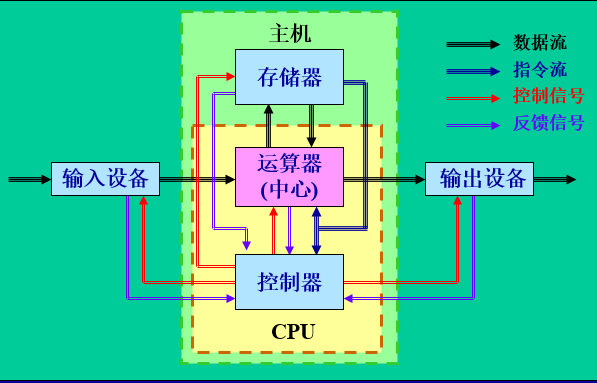
\includegraphics[width=1.0\textwidth]{img/计算机体系结构.png}

    \subsection{计算机各部件基本功能}
    \paragraph{CPU的基本功能:}

    ~

    根据程序执行所期望的信息处理,其中ALU执行算术逻辑运算,CU根据程序从存储器中读出并执行指令和数据,以执行要求的运算和操作。

    \paragraph{存储器的基本功能:}

    ~

    计算机存储指令、数据和信息的空间;

    \paragraph{输入输出设备的基本功能:}

    ~

    输入设备将指令、数据和信息输入到计算机,输出设备将处理后的结构由计算机输出出来。

    \subsection{计算机的指令系统}
    指令就是用以表示计算机微操作序列的二进制代码,它决定了CPU应该执行什么样的具体操作。

    操作系统就是一台计算机所能够执行的全部指令,在某种程度上,指令系统的完备与否以及功能强弱体现了计算机整体性能的优劣。同时,计算机设计中最基本的问题就是如何选择和设计出一个完备的、使用方便的指令系统。

    由于我们的出发点是在学习的基础之上加深对计算机的认识,以制作模型机为目标, 以期该计算机能够满足基本的运算操作,因此我们实际设计时不考虑指令系统的完备性,重点放在考察该系统的可用性。

    \subsection{计算机的工作原理}
    计算机的指令和数据都存储在存储器中,控制器每次从存储器中取出一条指令,它决定CPU应该执行什么样的操作具体操作,解释其含义,并据此产生一系列功能来执行此指令。

    处理一条指令所包含的操作序列称之为一个指令周期,其中,

    \qquad \qquad 指令周期 = 取值周期 + 执行周期。

    取指周期指的是将指令从存储器中读出的操作序列,执行周期由三部分构成,分别为指令译码、取操作数、完成操作。

    另外,值得注意的是,不同指令有不同字长、寻址方式、不同的操作,则其所对应的指令周期也长短不同。

    同时,每个指令周期划分为若干个机器周期,每个机器周期划分为若干个节拍,一个节拍通常对应一个时钟周期T,时钟周期是执行微操作的最小时间单位。

    \subsection{计算机的设计过程}
    计算机的设计可以分为两个阶段,分别为系统设计阶段和逻辑设计阶段。

    \paragraph{系统设计:} 设计系统的技术指标以及总的性能,确定设计目标、基本结构方案和指令系统。

    \paragraph{逻辑设计:} 将计算机结构的描述用逻辑电路来实现。
    \newpage

    \section{实验目的}
    我们希望通过我们数字逻辑的所学,以及查找相关的资料,按照典型计算机的实现原理来构建简易型的计算机,以满足基本的数据处理需要。

    同时,希望在学习实践制作中级计算机的过程中掌握数字逻辑设计的基本方法以及重要思想,在广泛查阅相关资料的基础之上对于现代化的许多硬件设计以及计算机设计方法有一个基本的了解,另外加深对于计算机体系结构的认识,为以后的学习研究打下坚实的基础。
    \newpage

    \section{实验原理}
    依据计算机设计实现的框图,该计算机设计与实现的基本原理大致步骤为:

    1. CLK脉冲进行数据输入,时钟计数器T-COUNTER产生时钟信号t;

    2. 设置PC指向00000000地址处,从此处开始取值;

    3. 将取得地址的低四位传递给IR进行译码,读出对应的执行指令;

    4. 根据logicProcess的组合逻辑,结合ti与qi算出对应的xi;

    5. 根据计算得到的xi进行相应的逻辑操作。
    \newpage

    \section{系统设计}
    综合考虑实际需要,该中级计算机系统将包括3个寄存器,分别为A,B和R。另外有多个译码器等(进行了器件的封装)。

    \subsection{存储器}
    每个存储器都是256个字,其中每个字8位;

    该存储器具有以下寄存器:

    \paragraph{存储地址寄存器MAR:} 与存储器的地址总线相连,存放着将要访问的存储单元的地址;

    \paragraph{存储缓冲寄存器MBR:} 与存储器的数据总线相连,存放着要写入或者刚从存储单元读出的信息。

    \qquad    如果读出的为: \textbf{指令 = 操作码部分 + 地址部分},则将操作码部分送至指令寄存器IR, 将保留在MBR中的地址部分发送至MAR。

    \qquad    如果读出的为:\textbf{操作数}, 则将其放在寄存器A和R中.

    \paragraph{程序计数器PC:} 存放的是后续指令的地址,且有计数功能。

    \paragraph{指令寄存器IR:} 存放的是现行指令的操作码。

    \paragraph{操作译码器:} 对指令寄存器IR提供的每个操作码译码出一个相应的输出变量$q_i$。

    \paragraph{时序译码器:} 提供计算机时序信号t1到t30这8个时钟信号。

    \paragraph{时序计数器:} 为计算机提供时序信号的计数器。

    以下为寄存器、存储器及其对应功能图表表示:

    \subsection{寄存器,存储器及其功能}
    \begin{table}
      \centering
      \begin{tabular}{|c|c|c|c|}
        \hline
        % after \\: \hline or \cline{col1-col2} \cline{col3-col4} ...
        符号 & 位数 & 名称 & 功能 \\
        \hline
        MAR & 8 & 存储地址缓存器 & 保存存储器地址 \\
        MBR & 8 & 存储缓冲寄存器 & 保存存储器内容 \\
        A & 8 & 寄存器A & 处理数据寄存器 \\
        B & 8 & 寄存器B & 处理数据寄存器 \\
        R & 8 & 寄存器R & 处理数据寄存器 \\
        PC & 8 & 程序计数器 & 保存指令地址 \\
        IR & 8 & 指令寄存器 & 保存指令操作码 \\
        T & 8 & 时序计数器 & 产生时序信号 \\
        \hline
      \end{tabular}
      \caption{寄存器及其功能}\label{寄存器及其功能}
    \end{table}
    \newpage

    \section{逻辑设计}
    \subsection{基本配置框图}
    为了制作一台简易计算机,总体的配置框图如下所示:

    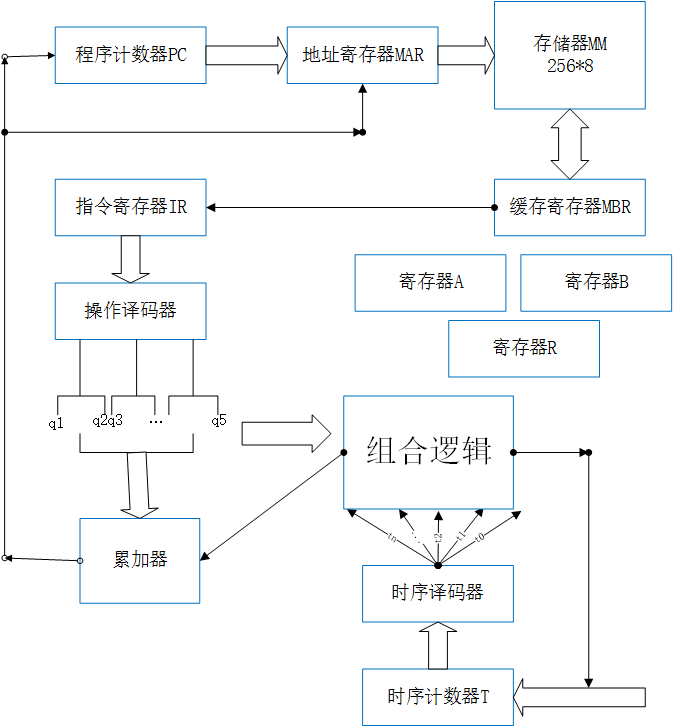
\includegraphics[width=0.6\textwidth]{./img/简易计算机配置框图.png}

    \subsection{时钟序列设计与实现}
    \paragraph{基本功能}

    ~

    时钟的基本功能是产生t0~29的时间控制序列,其由两个MSI计数器(74163)构成,其中由于仅有两输入,五输出,根据实际需要,仅仅使用级联全加器的低五位。

    \paragraph{单元输入与输出}

    \subparagraph{单元输入}

    ~

    1. CLK -- 时钟,上升沿触发使计数+1;

    2. RESET -- 当一条指令执行完毕之后进行t重置

    \subparagraph{单元输出}

    ~

    1. OUT1  -- 五位计数器的最高位

    2. OUT2 -- 五位计数器的第二高位

    3. OUT3 -- 五位计数器的第三高位

    4. OUT4 -- 五位计数器的第二低位

    5. OUT5 -- 五位计数器的最低位

    \paragraph{原理图}

    ~

    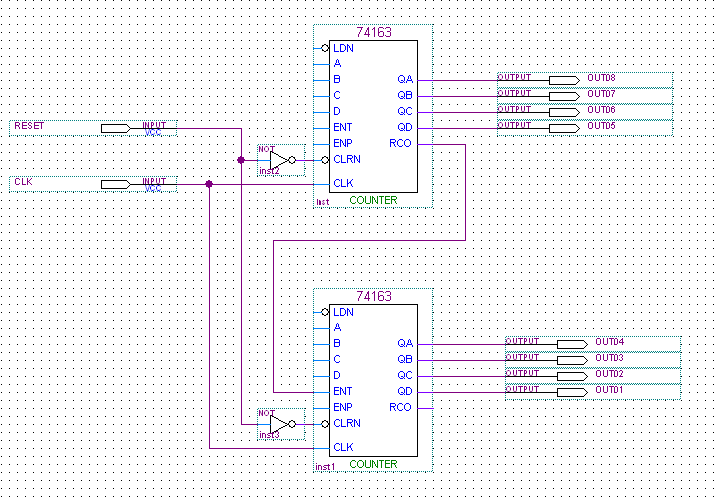
\includegraphics[width=0.8\textwidth]{./img/T-COUNTER原理图.png}

    \paragraph{封装逻辑图}

    ~

    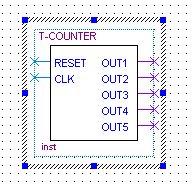
\includegraphics[width=0.4\textwidth]{./img/T-COUNTER封装逻辑图.png}

    \subsection{程序计数器PC设计与实现}
    \paragraph{基本功能}

    ~

    程序计数器PC是由8个D触发器构成的模256计数器,其实现的是进行RAM中地址指针的功能,根据逻辑需要可以进行+1操作。

    \paragraph{单元输入与输出}

    \subparagraph{单元输入}

    ~

    1. CLK -- 时钟脉冲,当上升沿触发PC计数+1

    \subparagraph{单元输出}

    ~

    1-7. Q0~Q7依次为PC指向地址的对应位的值(其中Q0--Q7升序排列)

    \paragraph{原理图}

    ~

    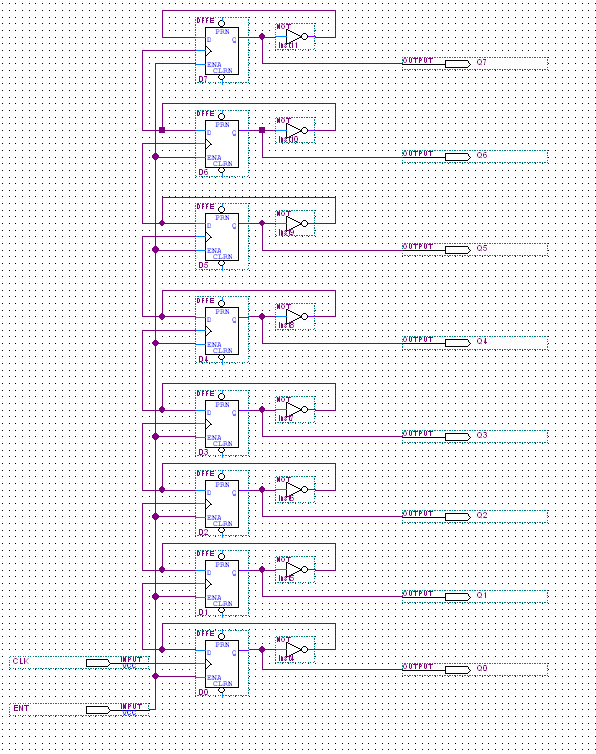
\includegraphics[width=0.8\textwidth]{./img/程序计数器PC原理图.png}

    \paragraph{封装逻辑图}

      ~

    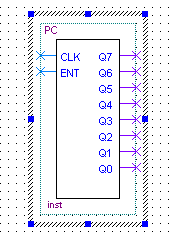
\includegraphics[width=0.4\textwidth]{./img/程序计数器PC封装逻辑图.png}

    \subparagraph{MAR, MBR设计与实现}
    \paragraph{基本功能}

    ~

    MAR是存储地址寄存器,MBR是存储数据寄存器。其中两种均通过74377进行实现,由于设计较为直接,因此没有进行封装。

    \paragraph{单元输入与输出}

    \subparagraph{单元输入}

    ~

    1. CLK -- 脉冲时钟,上升沿触发

    2. /EN -- 低使能有效

    3. D1~D8 -- 8位待存储数据地址

    \subparagraph{单元输出}

    ~

    1. Q1~Q8 -- 8为存储数据地址输出

    \paragraph{原理图}

    ~
    
    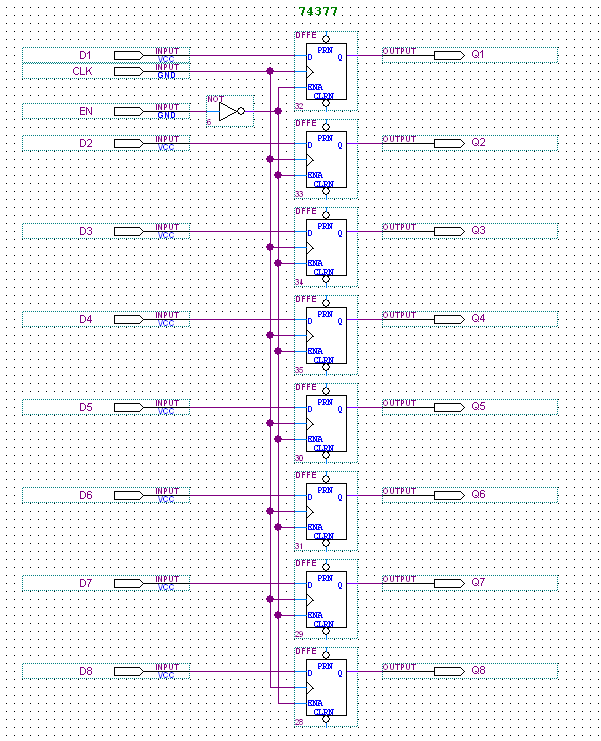
\includegraphics[width=1.0\textwidth]{./img/MAR,MBR原理图.png}

    \subsection{指令寄存器IR}
    \paragraph{基本功能}

    ~

    IR实现的功能是将从MBR得到的指令低四位进行译码(由于设计指令集的原因,10多条指令中只使用第四位就可以实现功能性译码)。然后将译码得到的值传送给logicPr2。

    \paragraph{单元输入与输出}

    \subparagraph{单元输入}

    ~

    1. OP1~OP4 -- 为指令的第四位(OP1--OP4按地址位升序排列)

    2. EN -- IR 指令译码使能控制

    \subparagraph{单元输出}

    ~

    输出为对应的指令,其中对应关系如下表所示:

    \begin{table}[!htb]
      \centering
      \begin{tabular}{|c|c|c|c|}
        \hline
        % after \\: \hline or \cline{col1-col2} \cline{col3-col4} ...
        操作码 & 助记符 & qi &执行功能 \\
        \hline
        0 0 0 0 0 0 0 0 & LDA addr & q1 & 将地址addr中的内容存入A寄存器处 \\
        0 0 0 0 0 0 0 1 & STA addr & q2 & 将A寄存器中的内容存入地址addr \\
        \hline
        0 0 0 0 0 0 1 0 & ADD addr & q3 & 将地址addr的内容加上A寄存器内容,存入A寄存器 \\
        0 0 0 0 0 0 1 1 & SUB addr & q4 & 将A中内容减去addr内容,并将结果存入A寄存器 \\
        \hline
        0 0 0 0 0 1 0 0 & AND addr & q5 & 将addr中内容与A寄存器中的内容进行与操作 \\
        0 0 0 0 0 1 0 1 & OR addr & q6 & 将addr中的内容与A寄存器中的内容进行或操作 \\
        \hline
        0 0 0 0 0 1 1 0 & MOV A, R & q7 & 将R中的内容存入A寄存器 \\
        0 0 0 0 0 1 1 1 & MOC B, R & q8 & 将R中的内容存入B寄存器 \\
        \hline
        0 0 0 0 1 0 0 0 & LDI A, OPRD & q9 & 将操作数存入A寄存器\\
        0 0 0 0 1 0 0 1 & LDI B, OPRD & q10 &  将操作数存入B寄存器\\
        \hline
      \end{tabular}
      \caption{简易计算机指令集}\label{简易计算机指令集}
    \end{table}

    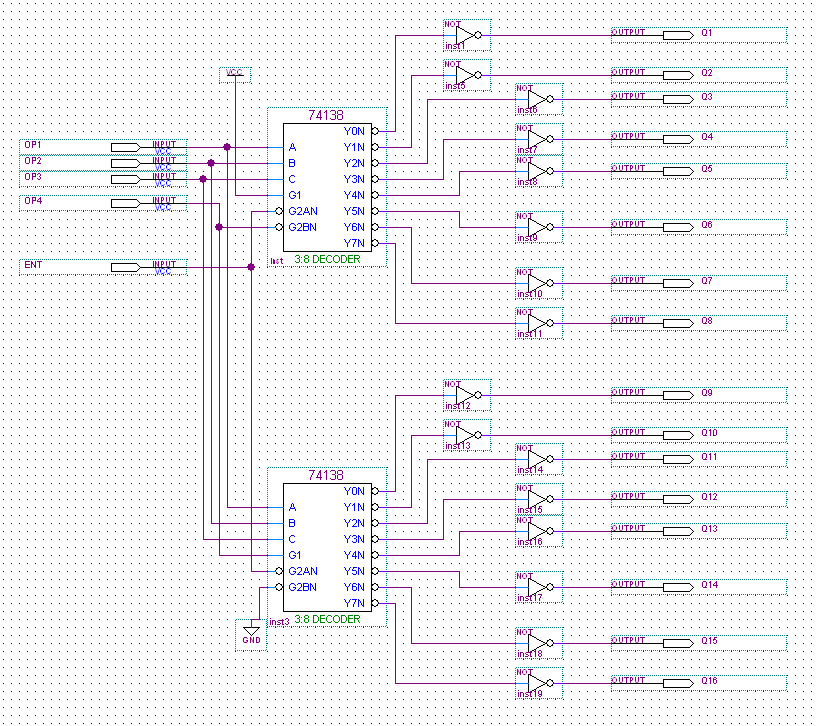
\includegraphics[width=1.0\textwidth]{./img/指令寄存器IR原理图.png}

    \paragraph{封装逻辑图}

    ~
    
    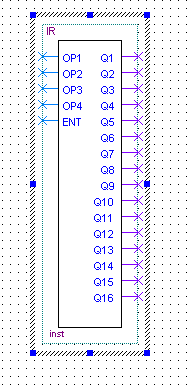
\includegraphics[width=0.4\textwidth]{./img/指令寄存器IR封装逻辑图.png}

    \subsection{寄存器A,B,R设计与实现}
    \paragraph{基本功能}
    分别实现三个数据寄存器的存储功能,由于A,B,R逻辑结构基本相同,因此综合进行分析。

    \paragraph{单元输入与输出}

    \subparagraph{单元输入}

    ~

    1. CLK -- 脉冲时钟,上升沿触发

    2. /EN -- 低使能有效

    3. D1~D8 -- 8位待存储数据地址

    \subparagraph{单元输出}

    ~

    1. Q1~Q8 -- 8为存储数据地址输出

    \paragraph{原理图}

    ~

    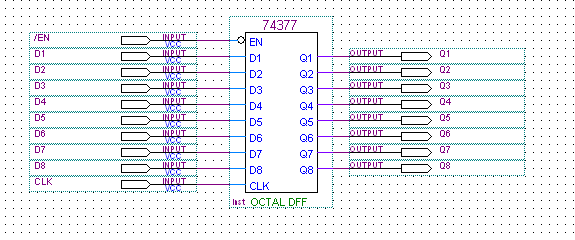
\includegraphics[width=1.0\textwidth]{./img/寄存器A,B,R原理图.png}

    \paragraph{封装逻辑图}

    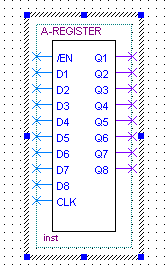
\includegraphics[width=0.4\textwidth]{./img/寄存器A,B,R封装逻辑图.png}

    \subsection{指令译码电路的设计与实现}
    \paragraph{基本功能}

    ~

    实现组合逻辑xi = qiti 的输出

    \paragraph{单元输入与输出}

    ~

    \subparagraph{单元输入}

    1. OP1~OP4 -- 待译码指令低四位

    2. B0~B4 -- 时钟序列t的二进制表示形式

    3. ENT -- 高使能

    \subparagraph{单元输出}

    1. x1~x29   根据逻辑实现的微操作序列

    \paragraph{原理图}

    由于原理图过大过于复杂,因此不在此处展示,详情参见代码。

    \paragraph{封装逻辑图}

    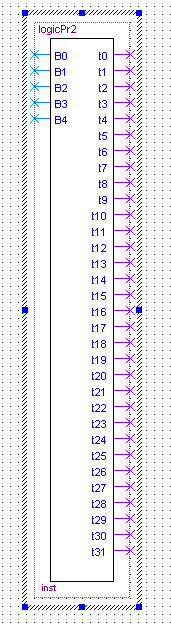
\includegraphics[width=0.4\textwidth]{./img/指令译码电路封装逻辑图1.png}

    \subsection{运算累加器设计与实现}
    我们累加器的实现使用8位JK触发器与组合逻辑电路进行实现,对于任何一个逻辑单元,具有如下的分析框图:

    ~

    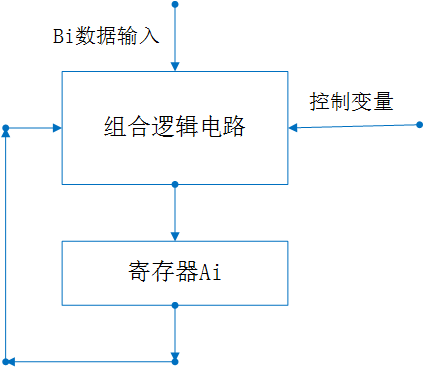
\includegraphics[width=0.6\textwidth]{../img/累加器基本结构.png}

    寄存器A既可以作为加数计数器,又可以作为和数计数器。决定累加器微操作的各个控制变量Pi是互斥的,在任何给定的时间内只有一个控制变量Pi被选通,产生相应的微操作。

    为简化累加器的设计,我们假设累加器由8个相同的单元组成,每个单元包含了执行各种微操作所需的逻辑电路,只要完成一个单元的各部分电路设计,就可以将他们综合成了累加器的一个典型单元,然后用若干个典型单元组成一个完整的累加器(迭代设计)。

    因此我们可以通过迭代的方式设置8个完整的逻辑单元。

    \subsection{RAM设计与实现}
    \paragraph{基本功能}

    ~

    存储数据及其地址的映射表。

    \paragraph{单元输入与输出}

    \subparagraph{单元输入}

    ~

    1. DATA1~DATA8 -- 写使能时读入的数据

    2. ADDR1~ADDR8 -- 传入的数据或指令地址

    3. WREN -- 读写使能控制,当WREN=1时,写使能,当WREN=0时,读使能;

    4. INCLK -- 输入时钟控制

    5. OUTCLK -- 输出时钟控制

    \subparagraph{单元输出}

    ~

    OUT1~OUT8 -- 指令或数据输出

    \paragraph{原理图}

    ~

    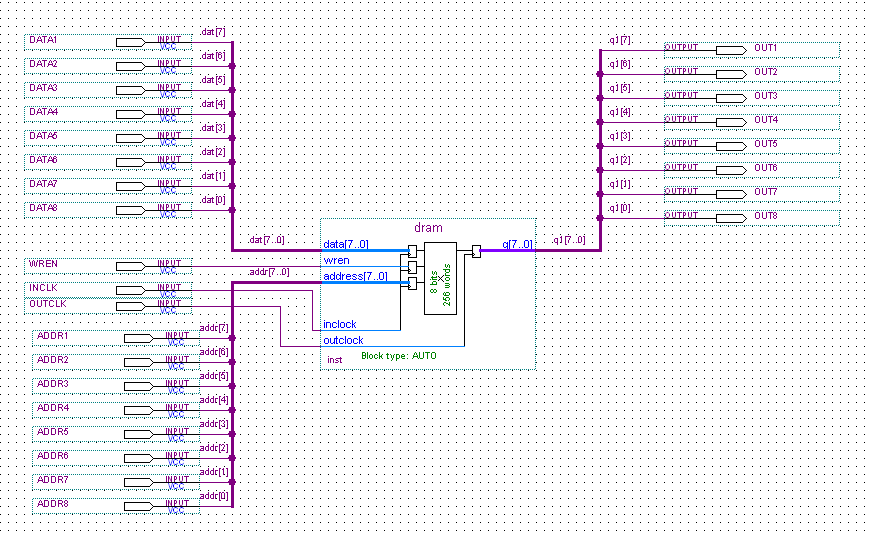
\includegraphics[width=1.0\textwidth]{img/RAM原理图.png}

    \paragraph{封装逻辑图}

    ~
    
    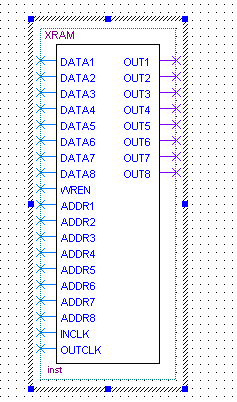
\includegraphics[width=0.4\textwidth]{img/RAM封装逻辑图.png}

    \newpage

    \section{实验平台}
    \subsection{实验设备}
    Cyclone II EP2C8T144C8试验箱.
    \subsection{实验器件}
    相关数据转换线,Win XP系统台式电脑, Ubuntu gnome 16.01 之下  Win 7虚拟机.
    \subsection{软件工具}
    QUARTER II 9.0, 截图工具, win系统画图软件, Latex texlive, Win Edt 10.2,  Sublime text 3, MiKTeX.
    \newpage

    \section{实验步骤及过程}
    \subsection{根据实验逻辑图完成模块设计并测试}
    我们将简易计算机的设计实现分为T计数器设计模块,A,B,R寄存器设计模块,logicProcess逻辑设计模块(包括IR和logicPr2两个部分的内容),PC模块,RAM模块,选择逻辑模块。该部分的具体内容已经在逻辑设计部分完成,详情参加逻辑设计部分。

    \subsection{逻辑模块的集成}
    将上述的多个模块集成在同一文件夹中,并且进行测试通过。

    其中,逻辑模块集成之后的逻辑结构图如下所示;

    ~

    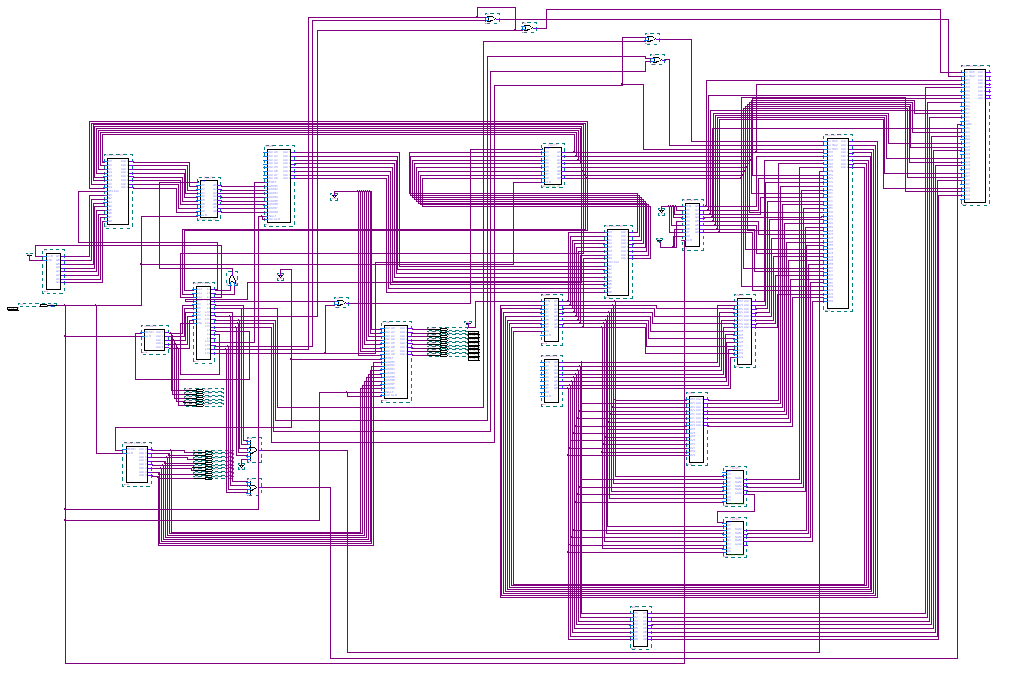
\includegraphics[width=1.0\textwidth]{./img/总体概览图.png}

    \subsection{计算机总逻辑图的编译与调试}
    经过反复测试与bug修正,结果表明,我们的计算机顺利地通过了编译与仿真。

    编译完成图片如图所示;

    ~

    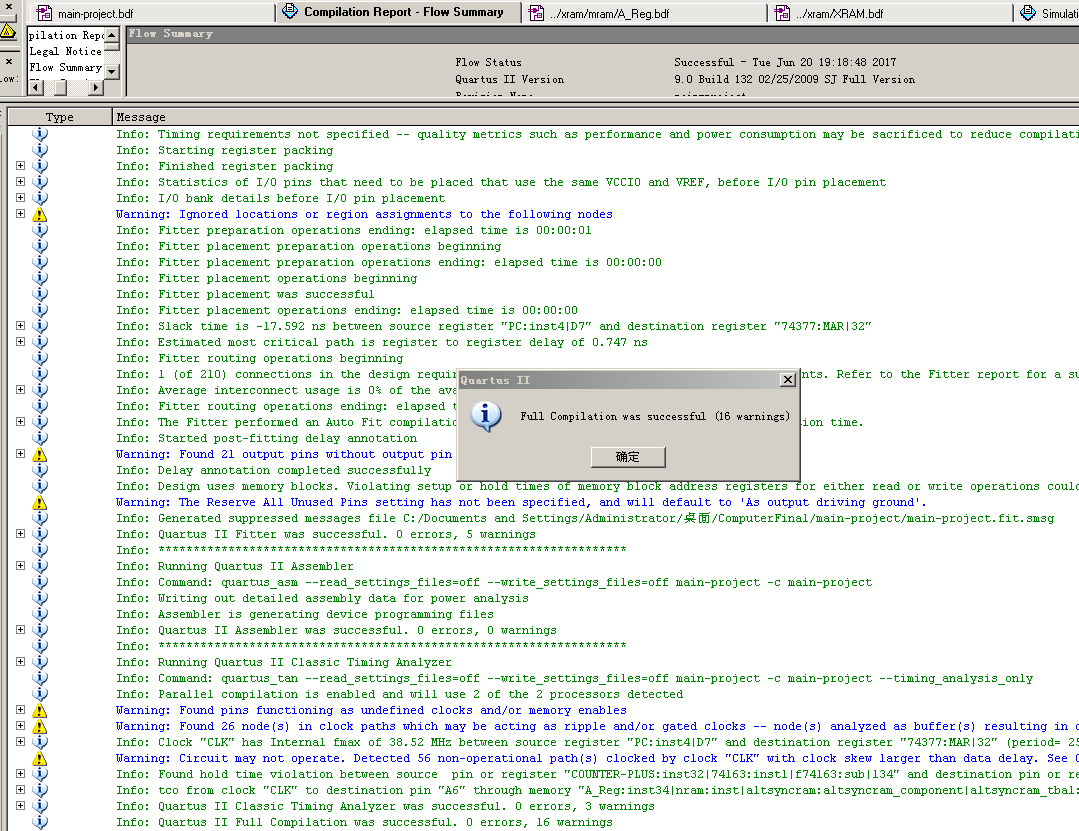
\includegraphics[width=1.0\textwidth]{./img/编译通过.png}

    仿真完成图片如图所示:

    ~

    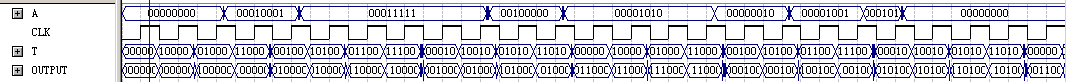
\includegraphics[width=1.0\textwidth]{./img/波形图1.png}

    以下是局部放大波形图:

    ~

    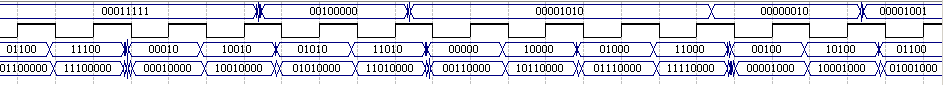
\includegraphics[width=1.0\textwidth]{./img/波形图2.png}

    ~

    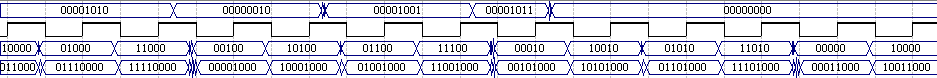
\includegraphics[width=1.0\textwidth]{./img/波形图3.png}


    \subsection{简易计算机的下载}
    计算机下载所使用的各输入输出端口以及其对应的引脚如图所示;

    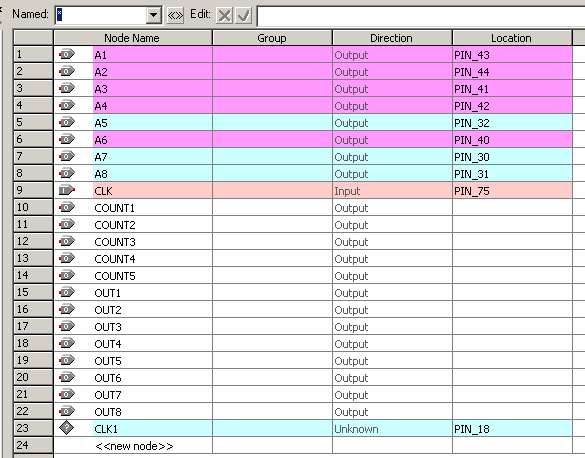
\includegraphics[width=1.0\textwidth]{./img/引脚使用.png}

    下载完成图片如图所示:

    ~

    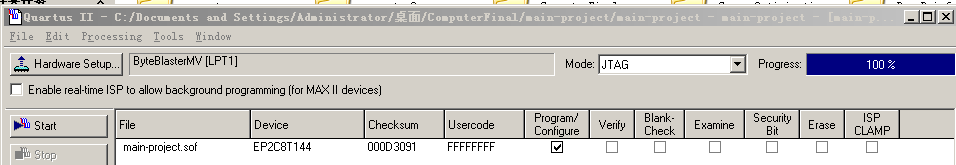
\includegraphics[width=1.0\textwidth]{./img/下载成功.png}

    \newpage

    \section{实验总结}
    小半个学期的《数字逻辑实验》课程的学习就这样结束了,同时也应该是张老师教给我们的最后一次课了。当时选定课题的时候,我们小组的五个人毅然决然地选择了计算机,而且有着种种不“简单”的想法,在这个过程去去不断地验证去学习,同时张老师提供了很多方向性的指导,一路走来,受益良多,感慨良多。

   	我将从\textbf{能力提升},\textbf{意识培养},\textbf{认识不足},\textbf{兴趣提升},\textbf{注重想法},\textbf{敢于开拓}这六个角度进行归纳总结:

   	\subsection{能力提升}
    虽然我们是软件工程专业的本科生,但是数字逻辑的学习过程中我们掌握了很多硬件设计的基本方法,同时在对于计算机设计实现的研究过程中,查阅了大量的相关资料,在这一路走来,能力,至少硬件设计以及搜索资料、获取资料的能力得到了较大提升。

   	\subsection{意识培养}
   	张老师以及毛老师上课反复强调,硬件设计是一种思维方法,是一种意识,是大家的按照硬件设计的基本流程进行分析问题,解决问题的意识,这种意识才是比知识更为重要的东西。老师在课堂之上循循善诱,逐步地引导我们对计算机、对硬件设计进行深入理解,同时又是如何去使用最简单的元器件进行硬件设计。在这个过程中,培养了我们的硬件分析与设计意识。

   	\subsection{认识不足}
   	在数字逻辑专题实验课程的学习过程中,这段经历总体而言是非常有趣的,很多的老师精选的例题不仅具有代表性,同时不乏趣味性,让我打开眼界,为之后的简易计算机的设计与实现,以及将来的硬件设计与应用的进一步学习奠定了坚实的基础。

   	在完成实验报告的过程中,总体思路经过了多次修正,硬件设计也经历了许多的曲折,而且在实际地单独对于某些问题进行系统分析的过程之中,发现实际上遇到了一些阻碍,同时也说明了自己的能力有待提升。虽然只是简易计算机的设计与实现,但是相对而言实际的计算机设计与实现,更具有挑战性,之后要加强这方面能力的提升以及强化训练。

   	\subsection{兴趣提升}
   	数字逻辑个人认为更多的是在兴趣驱动之下进行分析问题解决问题的过程,在这个过程中,遇到了很多新奇有趣的小技巧,同时也运用了许多让人眼前一亮的方法,极大地提升了自己进一步学习硬件设计,并提升数字逻辑设计能力的兴趣。

   	\subsection{注重想法}
   	数字逻辑的核心在于进行模块化的设计,同时在知晓全局的基础之上进行模块的实现,然后再将各个模块进行集成。往往好的模块规范决定了设计的成败与否,因此需要敢于去提出自己的想法,然后不断地修正,以期臻于完美。

   	\subsection{敢于开拓}
   简易计算机,或者说硬件设计的方法不是唯一的,或许能够得到满意的结果的都是合理化的方法,但是在这个过程中,如何加强工程化思想的渗透,同时设计得成一门艺术,则需要不断地去修正,不断地去开拓创新,这样才能够不断地完善简易计算机。

   	同时,其他课程以及科研训练的真谛也在于此,真正的魅力不在于我马上就可以找到解决问题的最好方法,而是在不断地摸索中,提升了个人的能力,培养了开拓创新的精神,这才是社会赖以生存发展的本质意义。
    \newpage

    \section{参考文献}
    [1] 鲍家元,毛文林,张琴. 《数字逻辑》(第三版). 高等教育出版社. 2011年11月.

    [2] 毛文林. 《数字逻辑课件》(第八章). 数字系统设计. 2017年4月.

    [3] 张琴. 《数字逻辑实验课件》. 西安交通大学. 2017年4月.

    [4] Intel® 64 and IA-32 Architectures Software Developer’s Manual. Volume 2 (2A, 2B, 2C and 2D): Instruction Set Reference, A-Z

    [5] 杜小智. 《嵌入式软件设计》. ARM指令集. 西安:西安交通大学. 2017年3月.

    [6] D.G.Meyer. Design of a Simple Computer. Introduction to Digital System Design. Purdue University.

        %$https://engineering.purdue.edu/ece270/Refs/supp_text_copyright_dgmeyer.pdf$.
    [7] Atera. https:\/\/www.atera.com\/faq

    [8] A Simple Computer. http:\/\/cs.lmu.edu\/~ray\/notes\/simplecomputer\/

    [9] Computer Design and Integration: CDI. http:\/\/www.cdillc.com\/
    \newpage

    \section{附录}
    \subsection{I: 简易计算机指令集}
    \begin{table}[!htb]
      \centering
      \begin{tabular}{|c|c|c|}
        \hline
        % after \\: \hline or \cline{col1-col2} \cline{col3-col4} ...
        操作码 & 助记符 & 执行功能 \\
        \hline
        0 0 0 0 0 0 0 0 & LDA addr & 将地址addr中的内容存入A寄存器处 \\
        0 0 0 0 0 0 0 1 & STA addr & 将A寄存器中的内容存入地址addr \\
        \hline
        0 0 0 0 0 0 1 0 & ADD addr & 将地址addr的内容加上A寄存器内容,存入A寄存器 \\
        0 0 0 0 0 0 1 1 & SUB addr & 将A中内容减去addr内容,并将结果存入A寄存器 \\
        \hline
        0 0 0 0 0 1 0 0 & AND addr & 将addr中内容与A寄存器中的内容进行与操作 \\
        0 0 0 0 0 1 0 1 & OR addr & 将addr中的内容与A寄存器中的内容进行或操作 \\
        \hline
        0 0 0 0 0 1 1 0 & MOV A, R & 将R中的内容存入A寄存器 \\
        0 0 0 0 0 1 1 1 & MOC B, R & 将R中的内容存入B寄存器 \\
        \hline
        0 0 0 0 1 0 0 0 & LDI A, OPRD & 将操作数存入A寄存器\\
        0 0 0 0 1 0 0 1 & LDI B, OPRD & 将操作数存入B寄存器\\
        \hline
      \end{tabular}
      \caption{简易计算机指令集}\label{简易计算机指令集}
    \end{table}
    \newpage

    \subsection{II: 内存地址及其对应指令(基础测试集1)}
    R上电输入00010101

    \begin{table}[!htb]
      \centering
      \begin{tabular}{|c|c|c|}
        \hline
        % after \\: \hline or \cline{col1-col2} \cline{col3-col4} ...
        地址 & 内容 & 说明 \\
        0000 0000 & 0000 0110 &  将R中的内容存入A寄存器\\
        0000 0001 & 0000 1001 &  将下一地址操作数存入B寄存器\\
        0000 0010 & 0000 1110 &  操作数为0000 1110\\
        0000 0011 & 0000 0010 &  将寄存器A与B的内容相加,结果存入A寄存器\\
        0000 0100 & 0000 0111 &  将R中的内容存入B寄存器\\
        0000 0101 & 0000 1000 &  将下一地址操作数存入A寄存器\\
        0000 0110 & 0011 1111 &  操作数为0011 1111\\
        0000 0111 & 0000 0011 &  将A寄存器内容减去B寄存器内容存入A寄存器\\
        0000 1000 & 0000 1000 &  将操作数存入A寄存器\\
        0000 1001 & 0000 1010 &  操作数0000 1010\\
        0000 1010 & 0000 1001 &  将操作数存入B寄存器\\
        0000 1011 & 0000 0011 &  操作数0000 0011\\
        0000 1100 & 0000 0100 &  将寄存器A与B内容相与存入A寄存器\\
        0000 1101 & 0000 1001 &  将操作数存入B寄存器\\
        0000 1110 & 0000 0101 &  操作数0000 1001\\
        0000 1111 & 0000 0101 &  将寄存器A与B内容相或存入A寄存器\\
        \hline
      \end{tabular}
      \caption{内存地址及其对应指令1}\label{内存地址及其对应指令1}
    \end{table}
    \newpage

    \subsection{III: 内存地址及其对应指令(基础测试集2)}
    R上电输入00010101

    \begin{table}[!htb]
      \centering
      \begin{tabular}{|c|c|c|}
        \hline
        % after \\: \hline or \cline{col1-col2} \cline{col3-col4} ...
        地址 & 内容 & 说明 \\
        \hline
        0000 0000 & 0000 0110 & 将R中内容(00010101)存入A寄存器\\
        \hline
        0000 0001 & 0000 1001 & 将下一个地址的操作数存入B寄存器 \\
        0000 0010 & 0001 1101 & 操作数00011101 \\
        \hline
        0000 0011 & 0000 0010 & 将寄存器A,B内容相加存入A寄存器 \\
        \hline
        0000 0100 & 0000 0000 & 进行LDA addr 操作 \\
        0000 0101 & 1000 0001 & 在地址1000 0001 取操作数 \\
        \hline
        0000 0110 & 0000 0011 & 将A,B 寄存器相减的内容存入A寄存器 \\
        \hline
        0000 0111 & 0000 1001 & 将下一个地址的操作数存入B寄存器\\
        0000 1000 & 0011 1100 & 操作数\\
        \hline
        0000 1001 & 0000 0100 & 将A, B寄存器中内容相与存入A寄存器 \\
        \hline
        0000 1010 & 0000 1000 & 将下一个地址操作数存入A寄存器 \\
        0000 1011 & 0000 0101 & 操作数\\
        \hline
        0000 1100 & 0000 0101 & 将A,B寄存器内容或运算,结果存入A寄存器\\
        \hline
        0000 1101 & 0000 1000 & 将下一个地址操作数存入A寄存器\\
        0000 1110 & 1111 1111 & 操作数\\
        \hline
        0000 1111 & 0000 1001 & 将下一个地址操作数存入B寄存器\\
        0001 0000 & 0101 0101 & 操作数\\
        \hline
        0001 0001 & 0000 0011 & 将A,B寄存器内容相减,结果存入A寄存器\\
        \hline
        --- & --- & --- \\
        \hline
        1000 0001 & 0000 0111 & 操作数0000 0111\\
        \hline
        --- & ---  & --- \\
        \hline
      \end{tabular}
      \caption{内存地址及其对应指令2}\label{内存地址及其对应指令2}
    \end{table}
    \newpage

    \subsection{IV: 微操作表}
    \begin{table}[!htb]
      \centering
      \begin{tabular}{|c|c|c|}
        \hline
        % after \\: \hline or \cline{col1-col2} \cline{col3-col4} ...
        时间序列 & 助记符号 & 注释\\
        \hline
        \textbf{标准取指令周期 }& &\\
        $t_0$ &  $MAR \Leftarrow PC$ & 传送指令地址 \\
        $t_1$ & Empty &  \\
        $t_2$ & $ MBR \Leftarrow M[MAR], /WREN, PC \Leftarrow PC + 1 $ & 读出操作码,且PC+1\\
        $t_3$ & Empty &  \\
        $t_4$ & Empty &  \\
        $t_5$ & $IR \Leftarrow MBR $ & 读出操作码,将其传给IR \\
        $t_6$ & Empty &  \\
        ---&---&---\\
        \hline
        \textbf{MOV A, R} & 将R中的内容存入A  & 使用q1进行控制\\
        $q_1t_7$ & $ A \Leftarrow R, T \Leftarrow 0 $& R内容存入A,同时T清零 \\
        $q_1t_8$ & Empty &  \\
        ---&---&---\\
        \hline
        \textbf{MOV B, R }& 将R中的内容存入B寄存器  & 使用q2进行控制\\
        $q_2t_7$ & $B \Leftarrow R, T \Leftarrow 0$ & R内容存入B,同时T清零 \\
        $q_2t_8$ & Empty &  \\
        ---&---&---\\
        \hline
      \end{tabular}
      \caption{微操作表1}\label{微操作表1}
    \end{table}
    \newpage

    \begin{table}[!htb]
        \centering
        \begin{tabular}{|c|c|c|}
        \hline
        % after \\: \hline or \cline{col1-col2} \cline{col3-col4} ...
        \textbf{LDI A, OPRD }& 将下一地址操作数存入A  & 使用q3进行控制\\
        $q_3t_7$ & $MAR \Leftarrow PC $& 操作数紧跟下一单元\\
        $q_3t_8$ & Empty &  \\
        $q_3t_9$ &$ MBR \Leftarrow M[MAR], /WREN, PC \Leftarrow PC + 1 $& 读操作数,PC+1 \\
        $q_3t_{10}$ & Empty &  \\
        $q_3t_{11}$ & Empty &  \\
        $q_3t_12$ & $A \Leftarrow MBR, T \Leftarrow 0$ & 传送操作数,同时T清零\\
        $q_3t_{13}$ & Empty &  \\
        ---&---&---\\
        \hline
        \textbf{LDI B, OPRD} & 将下一个地址操作数存入B  & 使用q4进行控制 \\
        $q_4t_7$ &$ MAR \Leftarrow PC$ & 操作数紧跟下一单元\\
        $q_4t_8$ & Empty &  \\
        $q_4t_9$ &$ MBR \Leftarrow M[MAR], /WREN, PC \Leftarrow PC + 1$ & 读操作数,PC+1 \\
        $q_4t_{10}$ & Empty &  \\
        $q_4t_{11}$ & Empty &  \\
        $q_4t_12$ & $B \Leftarrow MBR, T \Leftarrow 0 $& 传送操作数,同时T清零\\
        $q_4t_{13}$ & Empty &  \\
        ---&---&---\\
        \hline
        \hline
        \end{tabular}
    \caption{微操作表2}\label{微操作表2}
    \end{table}
    \newpage

    \begin{table}[!htb]
      \begin{tabular}{|c|c|c|}
        \hline
          % after \\: \hline or \cline{col1-col2} \cline{col3-col4} ...
        \textbf{AND A, B }& 将寄存器A和寄存器B内容相与存入寄存器A & 使用q5进行控制 \\
        $q_5t_7$ & $A \Leftarrow A and B , T \Leftarrow 0 $& \\
        $q_5t_8$ & Empty & \\
        $q_5t_9$ & Empty & \\
        $q_5t_{10}$ & Empty & \\
        ---&---&---\\
        \hline
        \textbf{OR A, B }& 将寄存器A和寄存器B内容相或存入寄存器A  & 使用q6进行控制 \\
        $q_6t_7$ & A $\Leftarrow A or B , T \Leftarrow 0$ & \\
        $q_6t_8$ & Empty & \\
        $q_6t_9$ & Empty & \\
        $q_6t_{10}$ & Empty & \\
        ---&---&---\\
        \hline
        \textbf{ADD A, B }& 将寄存器A和寄存器B内容相加存入寄存器A  & 使用q7进行控制\\
        $q_7t_7$ & $A \Leftarrow A + B , T \Leftarrow 0$ & \\
        $q_7t_8$ & Empty & \\
        $q_7t_9$ & Empty & \\
        $q_7t_{10}$ & Empty & \\
        ---&---&---\\
        \hline
        \textbf{SUB A, B }& 将寄存器A和寄存器B内容相减存入寄存器A  & 使用q8进行控制 \\
        $q_8t_7$ & $B \Leftarrow -B$ & 将B取反\\
        $q_8t_8$ & $Empty$ & \\
        $q_8t_9$ & $B \Leftarrow B + 1$ & 将B取补\\
        $q_8t_{10}$ & $Empty$ & \\
        $q_8t_{11}$ & $A \Leftarrow A + B , T \Leftarrow 0 $& \\
        $q_8t_{12}$ & $Empty$ & \\
        $q_8t_{13}$ & Empty & \\
        $q_8t_{14}$ & Empty & \\
        ---&---&---\\
        \hline
      \end{tabular}
      \caption{微操作表3}\label{微操作表3}
    \end{table}
    \newpage

    \begin{table}[!htb]
        \centering
        \begin{tabular}{|c|c|c|}
          \hline
          % after \\: \hline or \cline{col1-col2} \cline{col3-col4} ...
          \textbf{LDA ADDR} & 将地址addr中的内容存入A & 使用q9进行控制\\
          $q_9t_7$ & $MAR \Leftarrow PC$ & 将下一地址存入A中 \\
          $q_9t_8$ & Empty & \\
          $q_9t_9$ & $MBR \Leftarrow M[MAR], PC = PC + 1$ & 读操作数,PC+1\\
          $q_9t_{10}$ & Empty & \\
          $q_9t_{11}$ & Empty & \\
          $q_9t_{12}$ & $MAR \Leftarrow MBR$ & 传递操作数地址给MAR\\
          $q_9t_{13}$ & Empty & \\
          $q_9t_{14}$ & $MBR \Leftarrow M[MAR]$ & 读取操作数\\
          $q_9t_{15}$ & Empty & \\
          $q_9t_{16}$ & Empty & \\
          $q_9t_{17}$ & $A \Leftarrow MBR, T\Leftarrow 0$ & 传递操作数,转入T0取址\\
          $q_9t_{18}$ & Empty & \\
          ---&---&---\\
          \hline
          \textbf{STA ADDR} & 将A内容存入地址addr & 使用q10进行控制 \\
          $q_{10}t_7$ & $MBR \Leftarrow A$ & 将A寄存器内容存入MBR\\
          $q_{10}t_8$ & Empty & \\
          $q_{10}t_9$ & $MAR \Leftarrow PC$ & 将PC地址传给MAR\\
          $q_{10}t_{10}$ & Empty & \\
          $q_{10}t_{11}$ & $M[MAR] \Leftarrow MBR$ & 将MBR中内容写入MAR地址处\\
          $q_{10}t_{12}$ & Empty & \\
          $q_{10}t_{13}$ & Empty & \\
          \hline
        \end{tabular}
        \caption{微操作表4}\label{微操作表4}
      \end{table}
      \newpage

    \subsection{V: 集成化微操作序列}

    \begin{table}[!htb]
      \centering
      \begin{tabular}{|c|c|}
        \hline
        % after \\: \hline or \cline{col1-col2} \cline{col3-col4} ...
        \textbf{Xi} & \textbf{微操作序列} \\
        \hline
        $x_1=t_0+q_3t_7+q_4t_7+q_9t_7+q_{10}t_9$    &   $MAR\Leftarrow PC$\\
        \hline
        $x_2=q_9t_{12}                  $    &   $MAR\Leftarrow MBR$\\
        \hline
        $x_3=t_2+q_3t_9+q_4t_9+q_9t_9      $    &   $PC\Leftarrow PC+1$\\
        \hline
        $x_4=t_2+q_3t_9+q_4t_9+q_9t_9+q_9t_{14}$    &   $MBR\Leftarrow M[MAR]$\\
        \hline
        $x_5=q_3t_{12}+q_9t_{17}            $    &   $A\Leftarrow MBR$\\
        \hline
        $x_6=q_1t_7                   $    &   $A\Leftarrow R$\\
        \hline
        $x_7=q_1t_7+q_2t_7+q_3t_{12}+q_4t_{12}+q_5t_7+q_6t_7+q_7t_7+q_8t_{11}+q_9t_{17}$ & $T\Leftarrow 0$\\
        \hline
        $x_8=t_5                     $    &   $IR\Leftarrow MBR$\\
        \hline
        $x_9=q_{10}t_{11}                 $    &   $M[MAR]\Leftarrow MBR$\\
        \hline
        $x_{10}=t_2+q_3t_9+q_4t_9           $    &   $\/WREN$\\
        \hline
        $x_{11}=q_2t_7                  $    &   $B\Leftarrow R$\\
        \hline
        $x_{12}=q_4t_{12}                 $    &   $B\Leftarrow MBR$\\
        \hline
        $x_{13}=q_5t_7                  $    &   $A\Leftarrow AandB$\\
        \hline
        $x_{14}=q_6t_7                  $    &   $A\Leftarrow AorB$\\
        \hline
        $x_{15}=q_8t_7                  $    &   $B\Leftarrow \-B$\\
        \hline
        $x_{16}=q_8t_9                  $    &   $B\Leftarrow B+1$\\
        \hline
        $x_{17}=q_8t_{11}                 $    &   $A\Leftarrow A+B$\\
        \hline
        $x_{18}=q_{10}t_7                 $    &   $MBR\Leftarrow A$\\
        \hline
      \end{tabular}
      \caption{集成化微操作序列}\label{集成化微操作序列}
    \end{table}

\end{document} 